The fundamental laws of mechanics apply to race cars as they do to any other body. These laws relate, among others, the body's linear position, angular orientation and their time derivatives, resulting in translational and rotational changes. Their three-dimensional vector definitions are shown in equations \ref{eq:linear-quantities} and \ref{eq:angular-quantities}. To simplify the equations, a rigid body is assumed. This means, that deformations which occur in the vehicle during dynamic maneuvers are negligibly small or vanish. Therefore, points on the body maintain the same distance relative to each other at all times. Furthermore, a two-dimensional motion in the road plane can be assumed in many cases because the effects of vertical dynamics are negligible. The simplified equations for that case will also be shown.

\begin{subequations}\label{eq:linear-quantities}
\begin{alignat}{2}%
p &= \begin{bmatrix}p_x, p_y, p_z\end{bmatrix}^T \\%
v &= \begin{bmatrix}v_x, v_y, v_z\end{bmatrix}^T \\%
a &= \begin{bmatrix}a_x, a_y, a_z\end{bmatrix}^T \\%
\beta &= \arctan\left(\frac{v_x}{v_y}\right) \approx \frac{v_y}{v_x}%
\end{alignat}
\end{subequations}
\begin{subequations}\label{eq:angular-quantities}
\begin{alignat}{2}%
\varphi &= \begin{bmatrix}\phi, \theta, \psi\end{bmatrix}^T \\%
\omega &= \begin{bmatrix}\dot{\phi}, \dot{\theta}, \dot{\psi}\end{bmatrix}^T \\%
\alpha &= \begin{bmatrix}\ddot{\phi}, \ddot{\theta}, \ddot{\psi}\end{bmatrix}^T%
\end{alignat}
\end{subequations}

The linear \textit{position} $p$ of a body comprises a longitudinal component along the $x$-axis, a lateral component along the $y$-axis and a vertical component along the $z$-axis. Its first time derivative $v = \frac{dr}{dt}$ and second time derivative $a = \frac{d^2r}{dt^2}$ are the body's linear velocity and acceleration, respectively. The scalar magnitude $\norm{v}$ of the velocity is called speed. In vehicles, the arctangent of the ratio of lateral and longitudinal velocities, often approximated as just the ratio, is furthermore called the \textit{vehicle sideslip angle} $\beta$. We will use $p$ for positions in earth-fixed coordinates, and $r$ for positions in vehicle coordinates.

The angular \textit{orientation} $\varphi$ of a body can be described by the roll angle $\phi$ around the $x$-axis, the pitch angle $\theta$ around the $y$-axis and the yaw angle, or heading, $\psi$ around the $z$-axis. The angular velocity $\omega$ and acceleration $\alpha$ describe the element-wise time derivatives of these angles.


\subsection{Transformation of Linear Velocity}
Every motion of a rigid body can be decomposed into a linear and an angular component. All points on that body experience the same angular velocity at all times, i.e. $\omega^A = \omega^B$ for any two points $A, B$ on the body. Since we define the \gls{cog} as reference point of the vehicle coordinate system and therefore as center of every rotation, the \gls{cog} will never experience a linear velocity in vehicle coordinates. However, every other point will experience different linear velocities depending on their position $r$ relative to the center of rotation. If there is a non-zero angular velocity, equation \ref{eq:offcenter-velocity-3d} holds for any point $P$, assuming the velocity at the \gls{cog} is known. The expanded form can be found in appendix \ref{sec:appendix-transformation-linvel}.

% For SFII transformation
\begin{equation}\label{eq:offcenter-velocity-3d}%
v^P = v^{CG} + \omega \times r^P%
\end{equation}

This becomes easier to visualize when regarding the two-dimensional case, where $v_z$, $\dot{\phi}$ and $\dot{\theta}$ are disregarded, as shown in equation \ref{eq:offcenter-velocity-2d}.

\begin{equation}\label{eq:offcenter-velocity-2d}%
v^P%
= \begin{bmatrix}v_x^{CG} \\ v_y^{CG} \\ 0\end{bmatrix} + \begin{bmatrix}0 \\ 0 \\ \dot{\psi}\end{bmatrix} \times \begin{bmatrix}r_x \\ r_y \\ r_z\end{bmatrix}%
= \begin{bmatrix}v_x^{CG}-\dot{\psi} \cdot r_y \\ v_y^{CG}+\dot{\psi} \cdot r_x \\ 0\end{bmatrix}%
 \end{equation}

Let us regard the example scenario shown in figure \ref{fig:offcenter-velocity}, where the vehicle has a positive yaw rate and the vehicle is moving forward and to the left. Point $A$ is at the front left ($r_x > 0$, $r_y > 0$), while point $B$ is at the rear right ($r_x < 0$, $r_y < 0$). Due to the positive yaw rate, $A$ experiences a higher $v_y$ but lower $v_x$ than the \gls{cog}. $B$, on the other hand, experiences a higher $v_x$ but lower $v_y$ than the \gls{cog}. If the yaw rate were zero, all points would experience the same linear velocity.

\begin{figure}
	\centering
	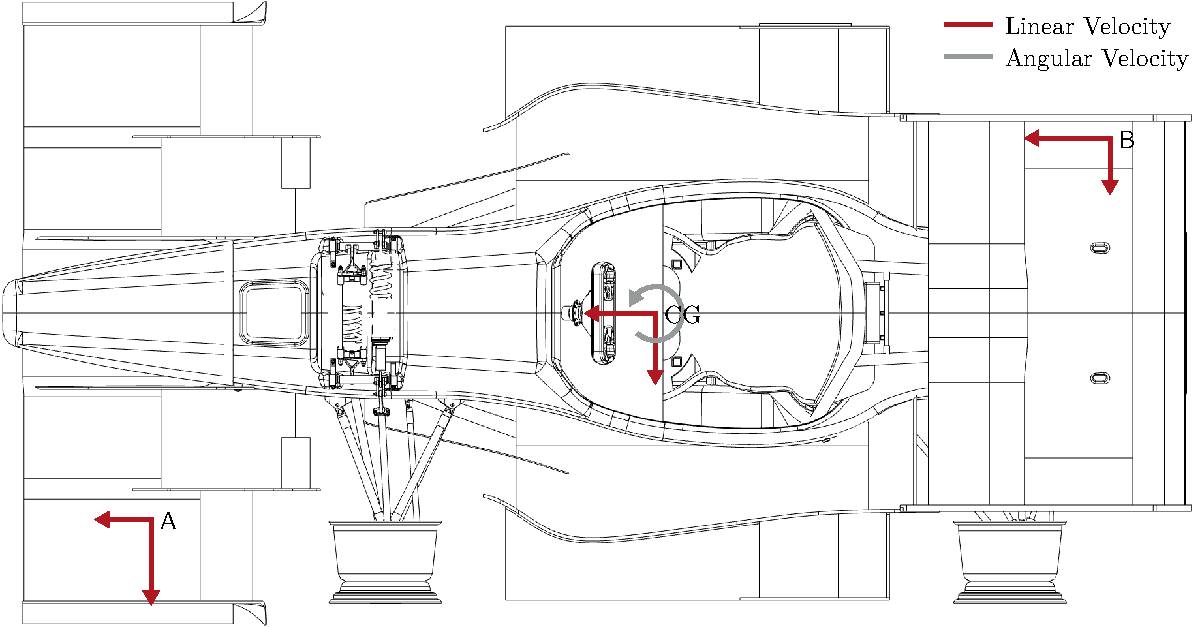
\includegraphics[width=\textwidth]{offcenter_velocity}%
	\caption{Experienced velocities at off-center points}
	\label{fig:offcenter-velocity}
\end{figure}


\subsection{Transformation of Linear Acceleration}
Like the angular velocity, the angular acceleration is the same at every point on a rigid body, i.e. $\alpha^A = \alpha^B$ for any two points $A, B$ on that body. However, these two points will generally not experience the same linear acceleration. Only if the rotational motion components $\omega$ and $\alpha$ are zero, the linear acceleration is equal for all points on the body, i.e. $a^A = a^B$. In the general case, equation \ref{eq:offcenter-acceleration-3d}~\cite[p.~140]{Gross.2014} holds for any point $P$ at location $r$. The expanded form can be found in appendix \ref{sec:appendix-transformation-linacc}.

\begin{equation}\label{eq:offcenter-acceleration-3d}%
a^P = a^{CG} + \alpha \times r^P + \omega \times (\omega \times r^P)%
\end{equation}

We can identify two additional components which affect the experienced linear acceleration. The term $\alpha \times r$ is the tangential acceleration along the circular path around the center of rotation, well known as $\alpha \cdot r$ in scalar notation. More significant due to the squared angular velocity, however, is the introduction of the centripetal acceleration $a_c$ in the term $\omega \times (\omega \times r)$. This term is the vector-equivalent of the acceleration resulting from the centripetal force $F_c$ as shown in equation \ref{eq:centripetal-acceleration} using the tangential velocity $v = \omega \cdot r$.

\begin{equation}\label{eq:centripetal-acceleration}%
F_c = \frac{mv^2}{r} \iff a_c = \frac{v^2}{r} = \omega^2 r%
\end{equation}

The two-dimensional form, shown in equation \ref{eq:offcenter-acceleration-2d}, is more intuitive than its three-dimensional counterpart. Here, $a_z$, $\dot{\phi}$, $\dot{\theta}$, $\ddot{\phi}$ and $\ddot{\theta}$ are assumed to be zero. The inward-direction of the centripetal effect can be seen by the negative signs of the angular velocity part.

\begin{equation}\label{eq:offcenter-acceleration-2d}%
a^P%
= \begin{bmatrix}a_x^{CG} \\ a_y^{CG} \\ 0\end{bmatrix}%
+ \begin{bmatrix}0 \\0 \\ \ddot{\psi}\end{bmatrix} \times \begin{bmatrix}r_x \\ r_y \\ r_z\end{bmatrix} \\%
+ \begin{bmatrix}0 \\ 0 \\ \dot{\psi}\end{bmatrix} \times \left(\begin{bmatrix}0 \\ 0 \\ \dot{\psi}\end{bmatrix} \times \begin{bmatrix}r_x \\ r_y \\ r_z\end{bmatrix}\right)%
= \begin{bmatrix}a_x^{CG}-\ddot{\psi} \cdot r_y-\dot{\psi}^2 \cdot r_x \\ a_y^{CG}+\ddot{\psi} \cdot r_x-\dot{\psi}^2 \cdot r_y \\ 0\end{bmatrix}%
\end{equation}

We demonstrate these effects in the example scenario shown in figure \ref{fig:offcenter-acceleration}, which is similar to the one in the previous subsection, but with an additional positive yaw acceleration. In point $A$, the tangential and centripetal acceleration cancel out and even surpass the linear acceleration experienced in the \gls{cog}, resulting in a negative $a_x$ and a much lower $a_y$. The opposite effect occurs in point $B$, where both $a_x$ and $a_y$ are amplified compared to the \gls{cog}.

\begin{figure}
	\centering
	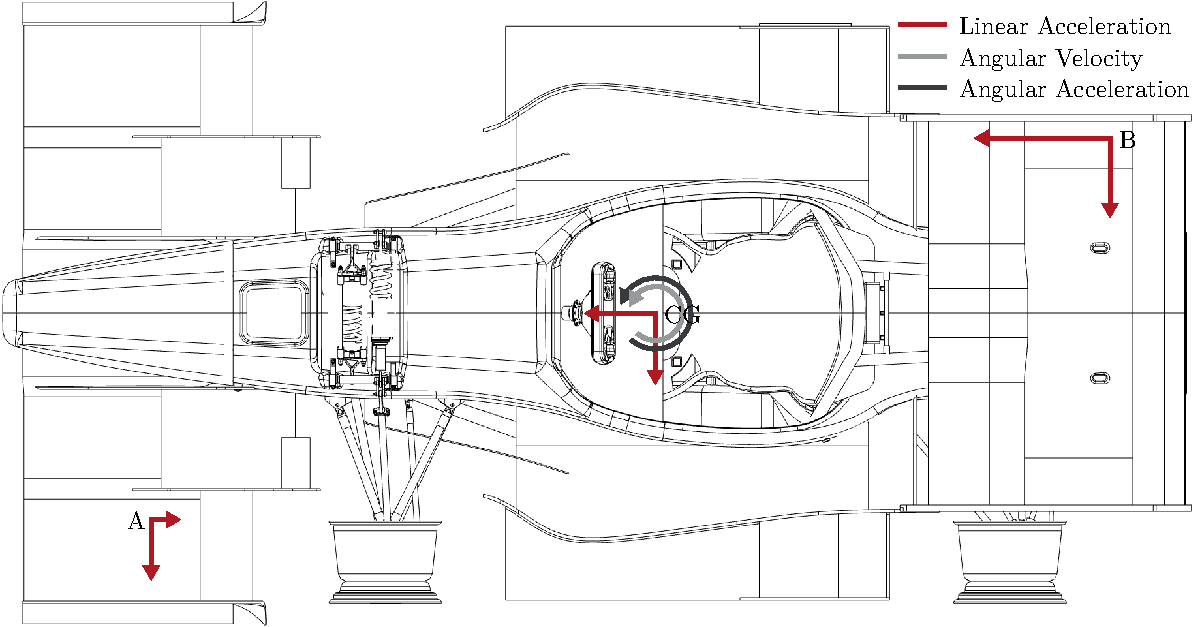
\includegraphics[width=\textwidth]{offcenter_acceleration}%
	\caption{Experienced acceleration at off-center points}
	\label{fig:offcenter-acceleration}
\end{figure}


\subsection{Calculation of Angular Acceleration From Linear Acceleration}
Direct measurement of the angular acceleration is often not possible. However, individual components of $\alpha$ can be calculated from the difference of two known linear acceleration vectors at different points $A, B$ with locations $r^A, r^B$ using equation \ref{eq:angacc-from-linacc-3d}. It is derived from equation \ref{eq:offcenter-acceleration-3d}, with $\Delta a = a^A - a^B$, $\Delta r = r^A - r^B$, and $a^{CG}$ being eliminated by the difference. The points must not be on the rotation axis of the calculated component of $\alpha$, otherwise they experience no angular acceleration. Thus, at least three non-collinear points are required to determine all components of $\alpha$. While the inverse of a cross product is not uniquely determined, as can be seen by the scalar factor $t$, $t = 0$ works well in practice.

\begin{equation}\label{eq:angacc-from-linacc-3d}%
\Delta a = \alpha \times \Delta r + \omega \times (\omega \times \Delta r) \implies%
\alpha = \frac{\Delta r \times (\Delta a - \omega \times (\omega \times \Delta r))}{\norm{\Delta r}^2} + t \cdot \Delta r, t \in \mathbb{R}%
\end{equation}

In two dimensions, this becomes easier to understand. Calculation of the yaw acceleration from the longitudinal and lateral accelerations of two points is shown in equation \ref{eq:angacc-from-linacc-2d}. We can see that the accelerations and distances from different axes are being correlated. The equation even shows how positioning both points on the $z$-axis would result in a zero division, which indicates that points off the rotation axis are required. When $A$ and $B$ are directly in front of and behind the \gls{cog} on the $x$-axis, i.e. $\Delta r_y = 0$, the equation simplifies to $\ddot{\psi} = \frac{\Delta a_y}{\Delta r_x}$. For practical applications, increasing the distance between the two points minimizes the effects of measurement uncertainty in the result.

\begin{equation}\label{eq:angacc-from-linacc-2d}%
\alpha%
= \frac{\begin{bmatrix}\Delta r_x \\ \Delta r_y \\ 0\end{bmatrix} \times \begin{bmatrix}\Delta a_x-\dot{\psi}^2 \cdot r_x \\ \Delta a_y-\dot{\psi}^2 \cdot r_y \\ 0\end{bmatrix}}{\begin{Vmatrix}\Delta r_x \\ \Delta r_y \\ 0\end{Vmatrix}^2}%
\implies \ddot{\psi} = \frac{\Delta r_x\Delta a_y - \Delta r_y\Delta a_x}{\Delta r_x^2 + \Delta r_y^2}%
\end{equation}


\subsection{Transformation of Velocity Between Coordinate Systems}\label{sec:background-transform-linvelocity}
Most sensor measurements are done in the vehicle coordinate system. Others, such as position measurements from a \gls{gnss} like GPS or Galileo, will be made in earth-fixed coordinates. To relate these, we need to be able to transform the vehicle velocity from the vehicle coordinate system to the earth-fixed coordinate system, which has an inertial, non-accelerating reference frame. Since \gls{gnss} altitude information are not relevant for our application, both coordinate systems can be thought of as parallel two-dimensional planes in three-dimensional space with the heading $\psi$ as mutual rotation. Equation \ref{eq:transform-linear-velocity} shows how the velocity can be transformed using a simple rotation, which effectively extracts the east-/northward components of the velocity vector in vehicle coordinates.

% For EKF position--velocity
\begin{equation}\label{eq:transform-linear-velocity}%
\begin{bmatrix}\prescript{E}{}{v}_x \\ \prescript{E}{}{v}_y\end{bmatrix}%
=\begin{bmatrix}cos(\psi) & -sin(\psi) \\ sin(\psi) & cos(\psi)\end{bmatrix}%
\begin{bmatrix}\prescript{V}{}{v}_x \\ \prescript{V}{}{v}_y\end{bmatrix}%
\end{equation}


\subsection{Calculation of Cornering Acceleration}\label{sec:background-cornering-acceleration}
The motion of a rigid body in the earth-fixed reference frame can be understood as a composition of a rotation and a translation, in our case with the \gls{cog} as center of rotation. In vehicles, this rotation results from cornering. The acceleration experienced in the \gls{cog} is the result of both the direct linear acceleration and the centripetal force resulting from the rotation, as shown in equation \ref{eq:cornering-acceleration}~\cite[p.~146]{Milliken.1996}. Other than in equation \ref{eq:offcenter-acceleration-3d}, the radius $R$ is not the distance to the \gls{cog} but the corner/curve radius. When driving straight, the radius approaches infinity and the centripetal force vanishes. Since $R$ is usually not known, we can substitute it using $R = v_{\perp} / \dot{\psi}$ with the tangential velocity $v_{\perp}$.

\begin{subequations}\label{eq:cornering-acceleration}
\begin{alignat}{3}%
a_x &= \dot{v}_x - \dot{\psi}^2 R &= \dot{v}_x - \dot{\psi}v_y \\%
a_y &= \dot{v}_y + \dot{\psi}^2 R &= \dot{v}_y + \dot{\psi}v_x%
\end{alignat}
\end{subequations}


\subsection{Calculation of Velocity From Motor Speeds}\label{sec:motorspeeds-to-velocity}
While there is a plethora of methods for measuring vehicle velocity, such as optical cross-correlation, radar and 5th wheel, they are too expensive for widespread use and only used as ground truth during vehicle development. Therefore, velocity estimation in many automotive applications is based mainly on motor or wheel speed measurements, which are readily available, especially in electric cars. Equation \ref{eq:wheelspeeds} shows arguably the simplest method to estimate the longitudinal velocity, involving only the dynamic tire radius $r_{dyn}$, the wheel speed $\omega_{wheel}$, the motor speed $\omega_{motor}$ and the motor-to-wheel ratio $i_{gear}$.

\begin{equation}\label{eq:wheelspeeds}%
v_x = \omega_{wheel} r_{dyn} = \frac{\omega_{motor}}{i_{gear}} r_{dyn}%
\end{equation}

This method can only be used for a crude approximation of the longitudinal velocity component. It falls short when the wheel slip, i.e. the relative motion of tire and road surface, increases or the tire even locks up and the wheel slip approaches infinity.

A simple improvement is averaging over all four wheels. Note that transforming each wheel's velocity into the \gls{cog} using equation \ref{eq:offcenter-velocity-3d} is not necessary, since wheels can be assumed to be distributed symmetrically, therefore averaging effectively eliminates the effect of off-center velocities. More advanced methods are presented in~\cite{Song.2002}. The authors present three approaches to augment wheel speed data with acceleration measurements during transient maneuvers with high slip. The first estimator uses equation \ref{eq:wheelspeeds} until a high-slip situation occurs, at which point acceleration measurements are integrated over time with the last wheel-based velocity as initial condition, switching back afterwards to prevent drift. The second estimator reduces noise through a Kalman filter which averages both measurements, weighted by a constant obtained with fuzzy logic. Finally, the third estimator reduces adverse effects of acceleration bias and an incorrect dynamic roll radius through regression.
